\documentclass{article}

\usepackage[dblblindworkshop]{neurips_2026}
\workshoptitle{Foundation Models for Temporal Systems}

\usepackage[utf8]{inputenc}
\usepackage[T1]{fontenc}
\usepackage{hyperref}
\usepackage{url}
\usepackage{booktabs}
\usepackage{amsmath}
\usepackage{amsfonts}
\usepackage{graphicx}
\usepackage{microtype}
\hypersetup{hidelinks}

\graphicspath{{figures/}{../../docs/figures/}}

\title{When Forecasting Skill Is a Reporting-Floor Statistic:\
A Leakage-Aware Evaluation of Orbital Conjunction Histories}

\author{Anonymous Author(s)}

\begin{document}

\maketitle

\begin{abstract}
Temporal forecasting benchmarks can reward a model for learning how a database records an outcome rather than how the underlying system evolves. We study this failure mode in the public ESA Collision Avoidance Challenge archive, where the task is to predict the final reported $\log_{10} P_c$ of an orbital conjunction from messages available before a fixed horizon. On 1,659 held-out events at 48 hours, XGBoost lowers mean absolute error (MAE) from 5.080 for persistence to 2.809, but its non-floor MAE worsens from 4.073 to 7.562. The gain is dominated by reports that later collapse to the archive floor of $-30$. On a matched cohort observed at 72, 48, 24, and 12 hours, learned skill beyond persistence decays from 4.49 to 0.03 MAE units, while the model is worse than persistence off the floor at every horizon. A validation-selected floor hurdle reaches MAE 2.109 yet has $F_2=0$ on the high-risk class. Split-conformal coverage reaches 90.1\%, but the resulting 21.03-unit interval is too wide to support the intended decision. These results show why temporal-system evaluation should separate observation-process artifacts, typical-case accuracy, tail decisions, and useful uncertainty before treating aggregate forecast error as evidence of real-world skill.
\end{abstract}

\section{Introduction}

Forecasting an evolving physical system from sparse, irregular reports is a natural temporal-learning problem, but the target can entangle physical evolution with the observation and reporting process. In satellite conjunction assessment, successive Conjunction Data Messages (CDMs) update geometry, covariance, and a reported collision probability $P_c$ as new tracking arrives~\citep{ccsdsCdm}. ESA's Collision Avoidance Challenge asks a model to predict the final reported $\log_{10} P_c$ using only messages available at least two days before closest approach~\citep{uriot2021,esaKelvins}. The target is a later estimate, not a collision outcome, and $-30$ is a database floor rather than a precisely observed probability.

This setting exposes an evaluation problem that matters for temporal foundation models even when the fitted predictors are deliberately conventional. A model may improve average error by detecting which records will be censored at a reporting floor, while becoming worse on ordinary non-floor cases and unsafe on the rare events that drive operational decisions. Scaling the temporal model does not resolve that mismatch; it can make the aggregate score more persuasive without making the forecast more useful.

We make three contributions. First, we construct event-disjoint, cutoff-safe histories and measure learned skill against persistence on the same events across four forecast horizons. Second, we decompose error by the target's point mass at the reporting floor and evaluate the scarce high-risk tail separately. Third, we test whether calibrated predictive uncertainty produces a usable abstention rule. The result is a negative but actionable benchmark diagnosis: history contains signal for floor membership, yet the tested learned policies do not improve non-floor forecasting or high-risk decision quality.

\section{Data and evaluation protocol}

The ESA archive contains 162,634 CDM rows from 13,154 anonymized events recorded during 2015--2019~\citep{esaKelvins,uriot2021}. An event is eligible when it has at least one message before the cutoff and a later labeled report, leaving 8,293 events at 48 hours. We split by event into 3,731 training, 1,659 validation, 1,244 calibration, and 1,659 test events. All feature extraction is performed after the cutoff filter. The released official test set ($n=2,167$) is joined to labels only after model and policy freeze. The public data lack dates and object-pair identifiers, so we cannot perform calendar or object-pair splits; we report a mission-grouped split and the official test as complementary checks.

Let $r$ be the latest pre-cutoff report and $y$ the final reported $\log_{10} P_c$. Persistence predicts $\hat y=r$. The main learned baseline is squared-error XGBoost over 234 cutoff-safe variables: the latest snapshot, summaries of earlier risk, miss-distance, speed, and observation trajectories, and covariance trends. A residual variant predicts $y-r$. A two-part hurdle first predicts whether $y=-30$, then applies a residual regressor trained on non-floor events; its threshold is chosen on validation. Split conformal prediction is calibrated on a separate split~\citep{lei2018}.

We report overall and floor-excluded MAE, median absolute error, paired bootstrap intervals for $\Delta\mathrm{MAE}=\mathrm{MAE}_{\mathrm{persist}}-\mathrm{MAE}_{\mathrm{model}}$, and a two-sided Wilcoxon test on paired absolute errors. For decision quality we use ESA's high-risk class $y\geq-6$ and challenge loss $L=\mathrm{MSE}_{HR}/F_2$~\citep{uriot2021}. Hyperparameters, split membership, the hurdle threshold, and the 90\% conformal operating point are frozen before test evaluation.

\section{Aggregate skill comes from the floor}

The test target has a point mass: 1,352 of 1,659 outcomes equal $-30$, and 55.6\% of reports do not move after the 48-hour cutoff. Persistence therefore has median absolute error zero. Figure~\ref{fig:anatomy} shows the exact-persistence spike and the long floor-collapse tail.

\begin{figure}[t]
  \centering
  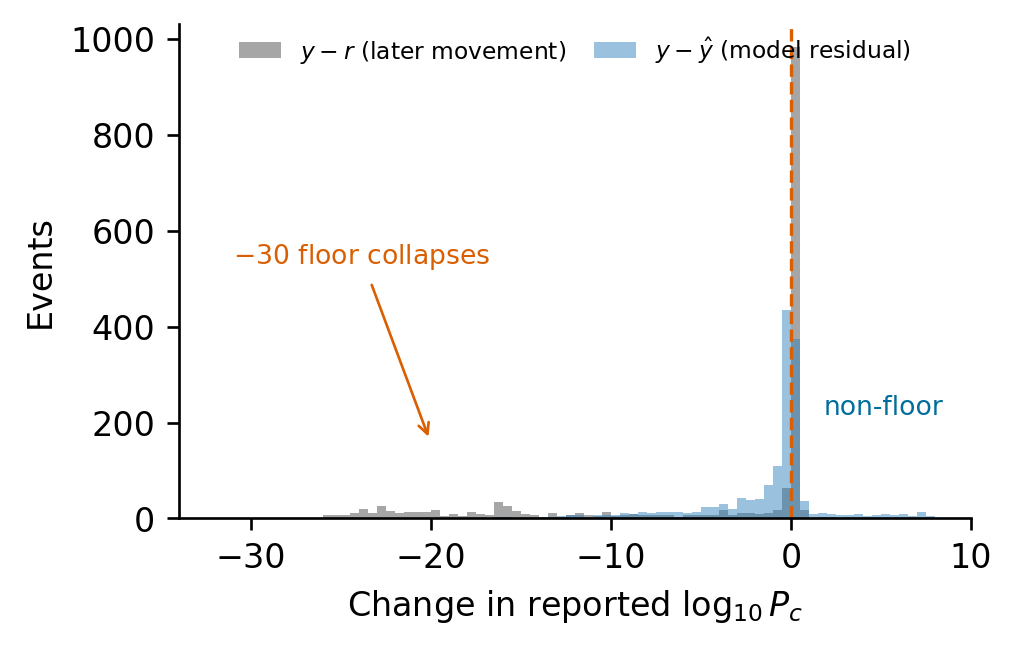
\includegraphics[width=0.80\linewidth]{error-anatomy-fmts.png}
  \caption{Later movement versus the unguarded XGBoost residual. Mean-error gains are concentrated in the left tail created by reports collapsing to the archive floor.}
  \label{fig:anatomy}
\end{figure}

Table~\ref{tab:main} gives the central decomposition. Unguarded XGBoost improves overall MAE by 2.270 units (95\% bootstrap interval $[1.930,2.638]$), but more than doubles error on non-floor events. Its paired absolute errors are not detectably better than persistence ($p=0.91$), because the mean gain is concentrated in large floor collapses. Predicting residuals does not change the conclusion. The hurdle produces the best overall MAE by calling the floor with high recall, but it also gives the worst non-floor MAE and no high-risk recall.

\begin{table}[t]
  \caption{Frozen local test at 48 hours ($n=1,659$; 1,352 floor events). Errors are in $\log_{10}P_c$ units.}
  \label{tab:main}
  \centering
  \small
  \begin{tabular}{lrrrr}
    \toprule
    System & MAE & Median & Non-floor & Floor \\
    \midrule
    Persistence & 5.080 & 0.000 & \textbf{4.073} & 5.308 \\
    Unguarded XGB & 2.809 & 0.554 & 7.562 & 1.730 \\
    Residual XGB & 2.760 & 0.453 & 7.375 & 1.712 \\
    Floor hurdle & \textbf{2.109} & \textbf{0.000} & 9.311 & \textbf{0.474} \\
    \bottomrule
  \end{tabular}
\end{table}

This behavior is robust to redefining the floor at $-20$ or $-25$: XGBoost remains worse than persistence after excluding the corresponding censored tail. A risk-only logistic model already predicts floor membership with test AUROC 0.799, while the full hurdle classifier reaches 0.920. The benchmark's easiest learned structure is therefore substantially visible in the current report itself.

\section{Skill decays, and the decision tail fails}

We compare horizons on a matched cohort of 1,459 test events observed at 72, 48, 24, and 12 hours, which holds target composition fixed. XGBoost's overall advantage falls from 4.487 MAE units at 72 hours to 0.029 at 12 hours, where the bootstrap interval includes zero (Figure~\ref{fig:horizon}). Non-floor $\Delta$MAE is negative at every horizon: $-3.86$, $-3.95$, $-2.67$, and $-1.70$. History is most informative early, but the information learned by this model is floor-collapse signal rather than general forecast improvement.

\begin{figure}[t]
  \centering
  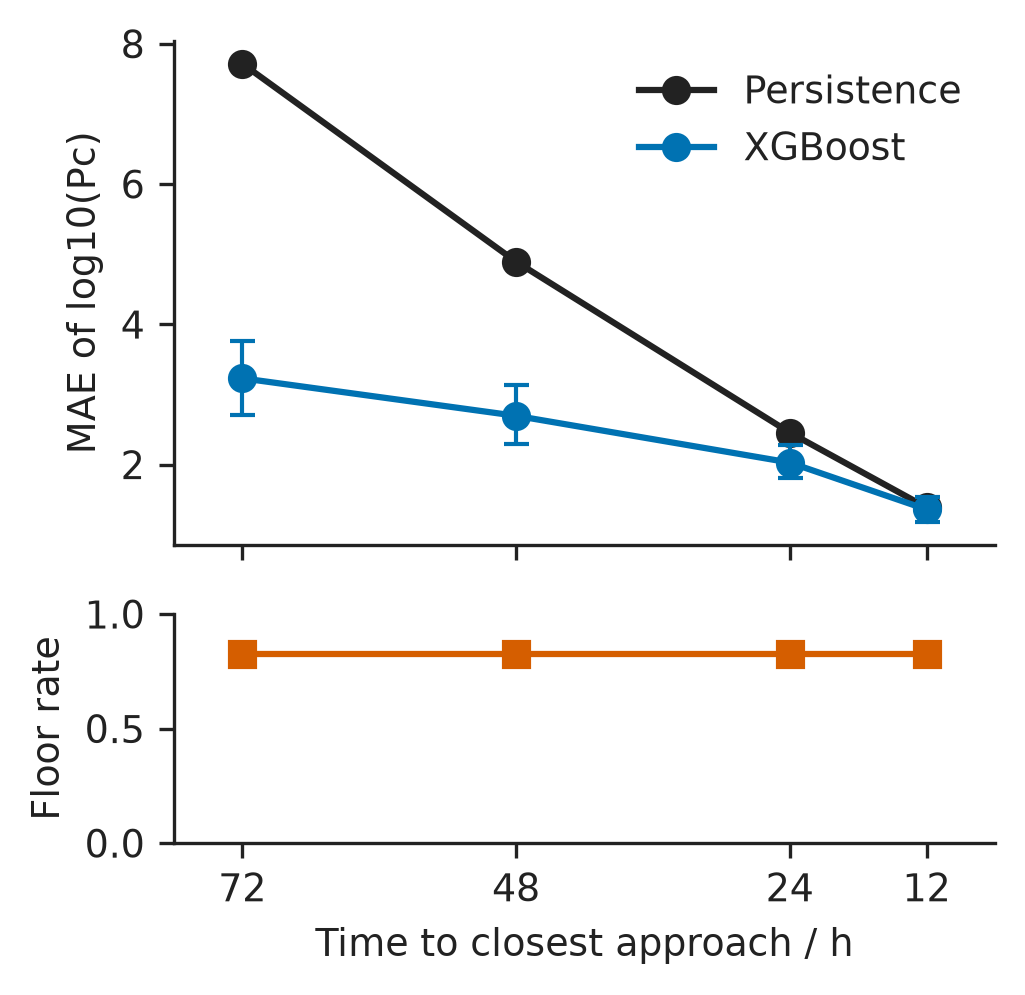
\includegraphics[width=0.80\linewidth]{horizon-decay.png}
  \caption{Matched-cohort error across forecast horizons. The same events are evaluated at every horizon; whiskers are 95\% bootstrap intervals.}
  \label{fig:horizon}
\end{figure}

The local test contains only nine high-risk events. Persistence has $F_2=0.361$, while unguarded, residual, and floor-hurdle policies all have $F_2=0$. In leave-one-high-risk-out evaluation across all 66 eligible high-risk events, persistence is closer than the residual model in 66 of 66 cases (mean absolute error 1.21 versus 12.59). On a mission-held-out split with 37 high-risk test events, XGBoost improves overall MAE (3.07 versus 4.74) but sharply worsens high-risk MAE (11.9 versus 1.50). The released official test confirms the decision mismatch: persistence obtains $L=0.694$, matching the published last-risk-prediction baseline, while unguarded XGBoost yields $F_2=0$ and $L\approx1.75\times10^6$ after an overconfident high-risk miss~\citep{uriot2021}.

\section{Calibrated does not mean useful}

The hurdle's 90\% split-conformal interval attains 90.1\% test coverage, but its constant width is 21.03 log units, wider than the gap from the archive floor to the $-6$ high-risk threshold. Coverage is 97.6\% on floor events and 57.0\% off the floor. An abstention rule that sends an event to review when its interval crosses $-6$ accepts 90.4\% of cases and lowers accepted-set MAE to 1.706, yet it still accepts two of nine high-risk events with forecasts below the threshold. At nominal coverage from 50\% through 80\%, the conformal radius is zero because most calibration residuals are exact floor hits. Marginal coverage is mathematically valid, but the mixture distribution makes it a poor certificate for the cases that matter.

\section{Implications for temporal-system evaluation}

This case study supports four evaluation requirements for models of evolving real-world systems. Benchmarks should identify censoring, clipping, imputation, and reporting floors before selecting an aggregate loss. They should compare against a strong time-local baseline on matched cohorts, because changing eligibility can masquerade as horizon-dependent skill. Typical cases and decision-critical tails require separate metrics when their frequencies and costs differ. Uncertainty should be judged by decision utility and subgroup coverage in addition to marginal calibration.

The findings do not show that temporal foundation models cannot help conjunction assessment. They show that this archive cannot support that claim through aggregate MAE alone. The data are historical and anonymized, object-pair leakage cannot be tested, manoeuvres are absent, and the target is a later report rather than a physical event. For this benchmark, a model chosen on MAE is chiefly a reporting-floor classifier; a model chosen on the operational loss would retain persistence or a persistence guard.

\clearpage
\bibliographystyle{plainnat}
\bibliography{references}

\appendix

\section{Additional results}

\subsection{Feature and model details}

The snapshot block contains 77 variables, the history block 68, and covariance trends 88 after encoding. The unguarded regressor uses 250 trees, learning rate 0.05, depth 4, minimum child weight 6, subsample 0.85, column sample 0.8, $\ell_1=0.1$, $\ell_2=2.0$, native missing-value handling, and seed 42. The floor classifier uses 180 depth-3 trees with train-set class weighting. Its threshold of 0.15 is selected on validation without a persistence guard. Across five grouped redraws, unguarded XGBoost's MAE advantage is $2.34\pm0.04$, while its floor-excluded MAE is $7.78\pm0.21$ versus $4.32\pm0.23$ for persistence.

\subsection{Official-test and selective-prediction details}

\begin{table}[h]
  \caption{Frozen official test ($n=2,167$; 150 high-risk; 1,673 floor).}
  \centering
  \small
  \begin{tabular}{lrrrrr}
    \toprule
    System & MAE & Median & Non-floor & $L$ & $F_2$ \\
    \midrule
    Persistence & 5.209 & 0.000 & 4.287 & 0.694 & 0.739 \\
    Unguarded XGB & 3.504 & 0.690 & 9.333 & $1.75\!\times\!10^6$ & 0.000 \\
    Residual XGB & 3.476 & 0.594 & 9.289 & 104 & 0.017 \\
    Floor hurdle & 3.177 & 0.000 & 11.832 & 70.5 & 0.025 \\
    Guarded ensemble & 3.107 & 0.439 & 6.750 & 0.694 & 0.739 \\
    \bottomrule
  \end{tabular}
\end{table}

\begin{table}[h]
  \caption{Conformal abstention on the local test. False reassurance (FR) counts accepted forecasts below $-6$ whose outcome is at least $-6$.}
  \centering
  \small
  \begin{tabular}{rrrrr}
    \toprule
    Nominal & Abstained & Accepted & Accepted MAE & FR \\
    \midrule
    50--80\% & 0 & 1.000 & 2.109 & 9/9 \\
    88\% & 80 & 0.952 & 1.812 & 5/9 \\
    90\% & 159 & 0.904 & 1.706 & 2/9 \\
    95\% & 166 & 0.900 & 1.689 & 2/9 \\
    \bottomrule
  \end{tabular}
\end{table}

\section{Reproducibility, data, and ethics statements}

\paragraph{Reproducibility.} The supplementary artifact contains frozen split identifiers, feature definitions, model hyperparameters, evaluation code, and scripts for every figure and table. The anonymous review package omits identifying repository links; a public link will be restored after review.

\paragraph{Data availability.} Inputs and labels come from the ESA Collision Avoidance Challenge dataset on Zenodo (DOI: \href{https://doi.org/10.5281/zenodo.4463683}{10.5281/zenodo.4463683}). The data remain subject to ESA's terms.

\paragraph{Ethics and intended use.} This retrospective study uses anonymized machine-generated conjunction records and involves no human participants. The models forecast later reported risk estimates and are not validated for manoeuvre decisions, live catalogues, or safety-critical deployment.

\paragraph{Funding, conflicts, and contributions.} Funding, conflicts of interest, author contributions, and acknowledgements are withheld during double-blind review and will be supplied in the camera-ready version.

\paragraph{Use of AI tools.} The authors used an AI assistant for manuscript editing and LaTeX preparation. The author verified the analyses, numerical claims, citations, and final text and remains responsible for the submission.

\end{document}
